\newpage
\section{Question 3}
	\subsection*{DH Notation}
	\noindent
		\begin{table}[position = here]
		\begin{centering}
		\begin{tabular}{||l|l|l|l|l||}

		\end{tabular}\\
		\end{centering}
		\begin{flushleft}
		\caption [DHVariables] {D-H Variable Notation}
		\end{flushleft}
		\end{table}
		
		
		\begin{figure}[position = here]
			\begin{centering}
				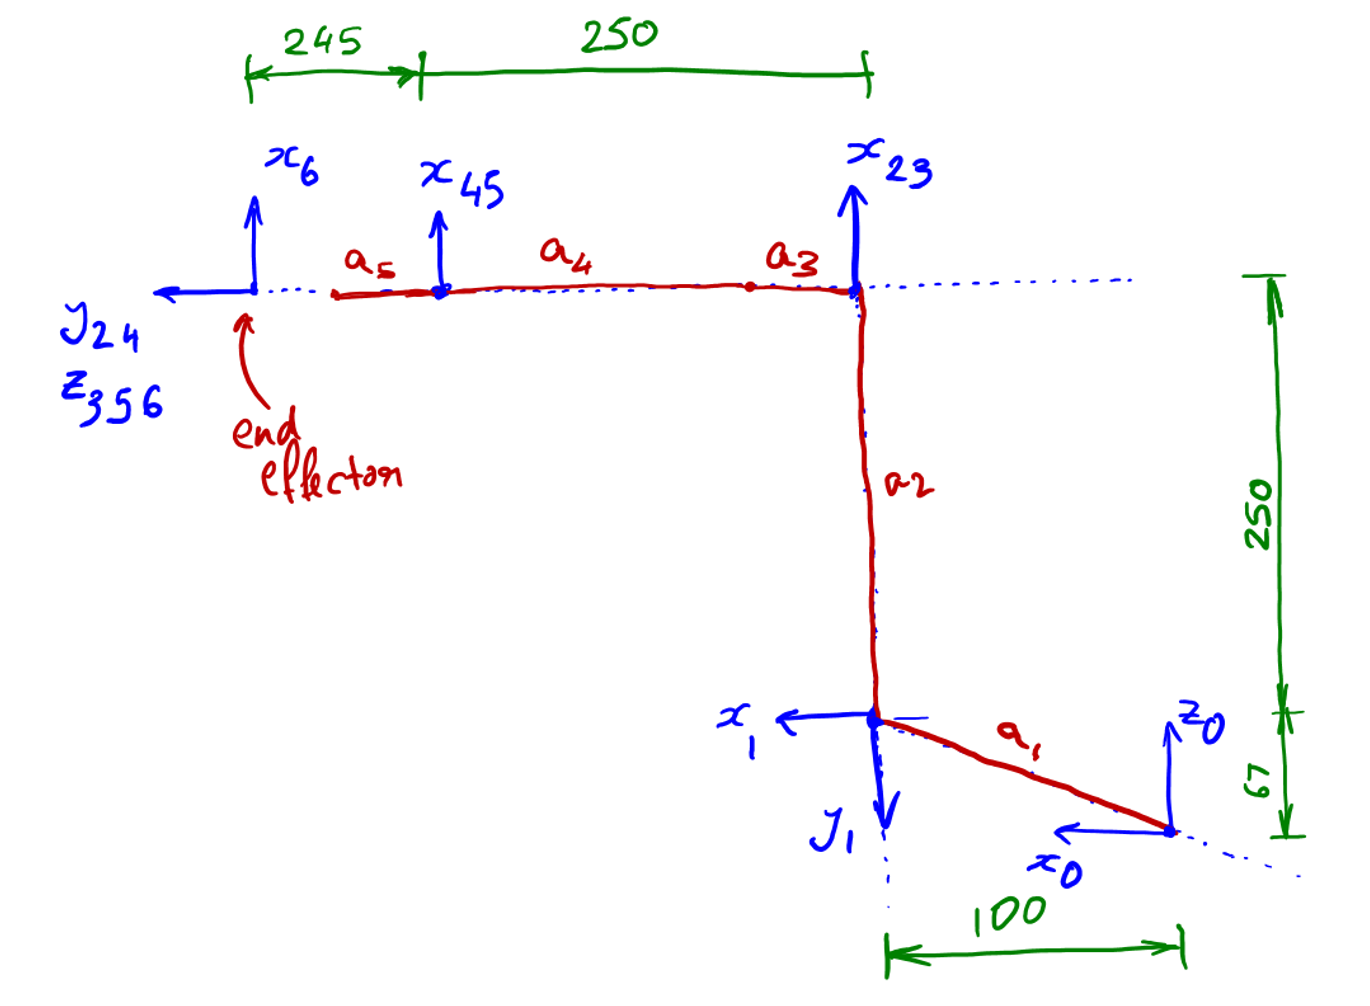
\includegraphics[scale=0.5]{q3}\\
			\end{centering}
		\end{figure}
		
	\pagebreak
	\subsection*{Assumption}

	\subsection*{Code Listing}
	See Appendix A [9.3]
	
	\subsection*{Resulting Transformation Matrix}
